    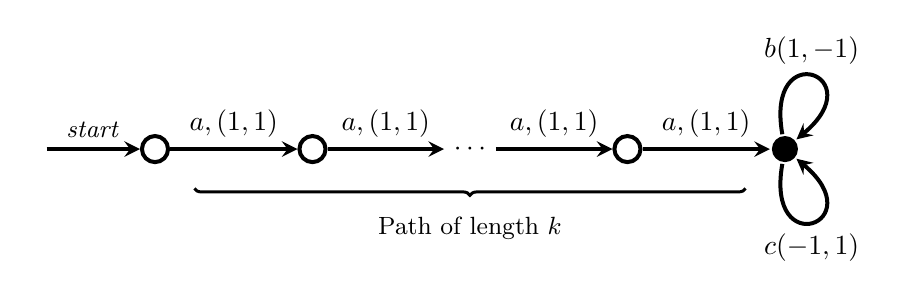
\begin{tikzpicture}
        \node (qs) at (-1.5, 0) {};
        \node[draw, circle, minimum size = 0.1in, line width = 0.02in] (q1) at (0,0) {};
        \node[draw, circle, minimum size = 0.1in, line width = 0.02in] (q2) at (2,0) {};
        \node (q3) at (4,0) {$\cdots$};
        \node[draw, circle, minimum size = 0.1in, line width = 0.02in] (q4) at (6,0) {};
        \node[fill, circle, minimum size = 0.1in, line width = 0.02in] (qf) at (8,0) {};

        \draw[-stealth, line width = 0.02in] (qs) -- node[above] {\small\textit{start}} (q1);
        \draw[-stealth, line width = 0.02in] (q1) -- node[above] {$a, (1, 1)$} (q2);
        \draw[-stealth, line width = 0.02in] (q2) -- node[above] {$a, (1, 1)$} (q3);
        \draw[-stealth, line width = 0.02in] (q3) -- node[above] {$a, (1, 1)$} (q4);
        \draw[-stealth, line width = 0.02in] (q4) -- node[above] {$a, (1, 1)$} (qf);
        \draw[-stealth, line width = 0.02in] (qf) edge[loop above, distance = 0.5in, out=100, in=40] node[above] {$b(1, -1)$} (qf);
        \draw[-stealth, line width = 0.02in] (qf) edge[loop below, distance = 0.5in, out=260, in=320] node[below] {$c(-1, 1)$} (qf);

        \draw[line width = 0.015in, decoration={brace, mirror}, decorate] (0.5, -0.5) -- (7.5, -0.5);
        \node at (4, -1) {\small Path of length $k$};
\end{tikzpicture}